En esta sección se van a evaluar los entornos de desarrollo más populares: React, Svelte, VueJS, Preact y Angular. Como preámbulo, se muestra en la figura \cref{fig:stjs2019:frontend} la satisfacción de los usuarios con respecto a cada entorno. Esto es relevante porque la satisfacción de los usuarios depende de factores como la eficiencia de código y la curva de aprendizaje. Como queremos que nuestro marco de trabajo esté destinado a aplicaciones pequeñas que tienen potencial para crecer, es importante conocer cuál es la opinión media de los usuarios de 2019. Además queremos que el entorno sea accesible al mayor número de usuarios, por lo que la popularidad es el factor más relevante en este estudio. 

\begin{figure}
	\centering
	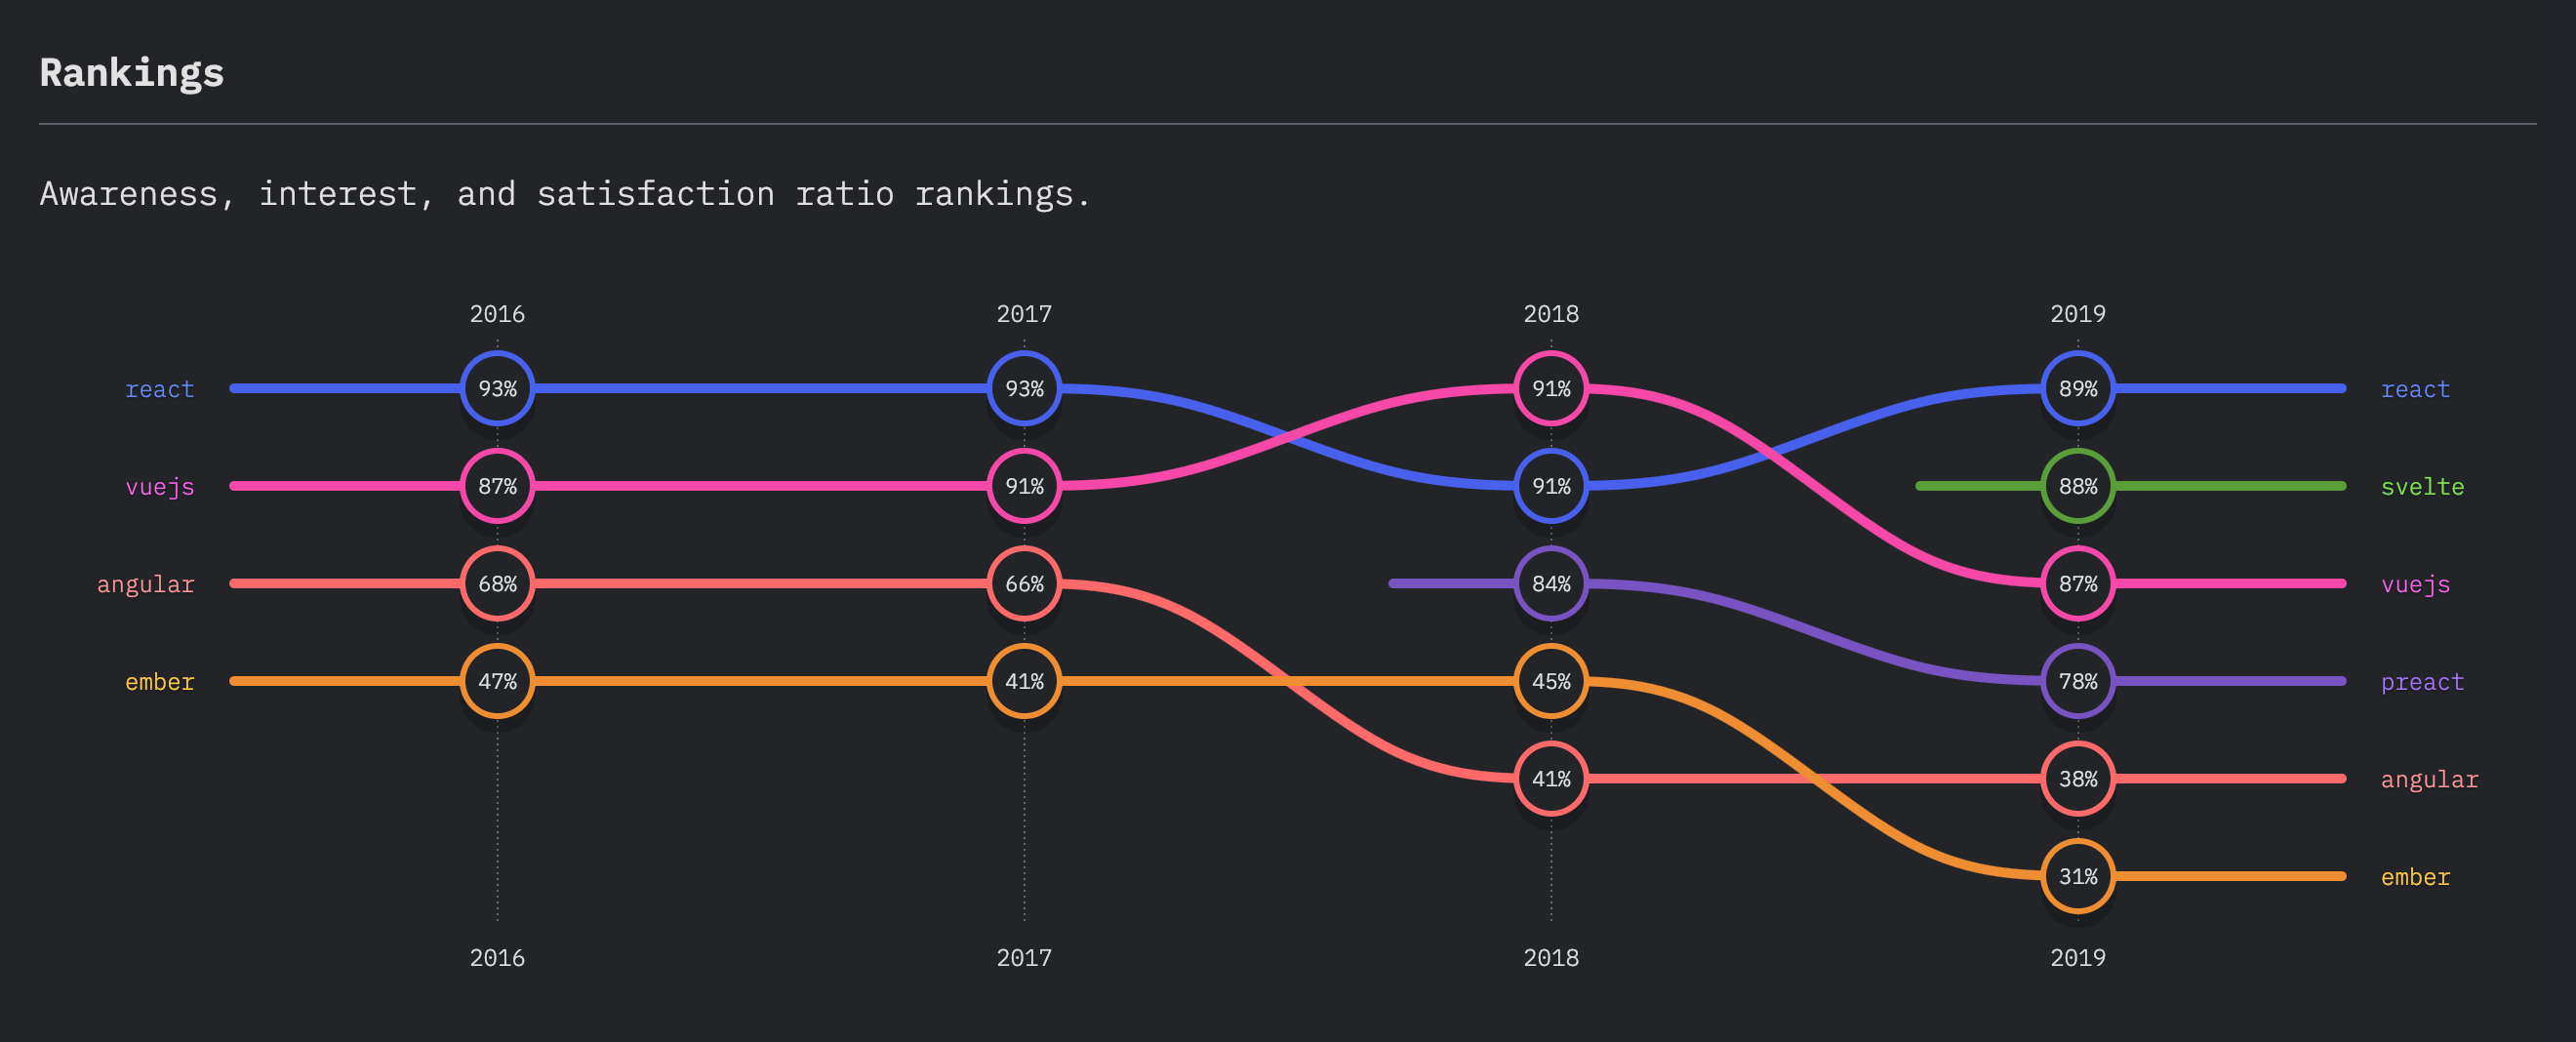
\includegraphics[width=\textwidth]{front_end_frameworks_experience_ranking.png}
	\caption{2019 - Opinión popular de los entornos de trabajo front-end}
	\label{fig:stjs2019:frontend}
\end{figure}

Parece que los dos más importantes en este sentido son React y VueJS (Svelte lo voy a descartar por el poco tiempo en el mercado). Según la comparación de rendimiento que presenta \citet{RWC2019} en su artículo, Vue parece líder en aplicaciones ligeras y rápidas. Por otro lado, en la comparativa que desarrolla \citet{TJSF2019}, se puede apreciar que React es utilizado por un 64.8\% de los desarrolladores web contra los 28.8\% que están con Vue. Además, React cuenta con más soporte y documentación que respaldan sus años de presencia en el mercado, mientras que la para floja de Vue hoy por hoy es su soporte.

Hay otro análisis a tener en cuenta para realizar esta elección, y es la facilidad para depurar el código. La limpieza, la cantidad de líneas y las herramientas de pruebas disponibles cumplemn un papel clave en este trabajo. Para valorarlo, he tenido en cuenta un artículo de \citet{RVVCTOG} que hace la comparativa desde el punto de vista de la calidad de código.

1. Tipado: Sabemos que Javascript no es un lenguaje tipado. Sin embargo, cuando hablamos de pruebas, es importante comprobar el tipo de los datos que fluyen a través de la aplicación. Tanto React como Vue permiten comprobaciones de tipos mediante Javascript tipado: TypeScript es una solución global al problema. Sin embargo, es más sencillo usar TypeScript en React. Además, React dispone de una herramienta oficial, Flow, que permite hacer estas comprobaciones de forma todavía más fácil.
2. Modularidad: Ambos entornos están basados en modularidad de código. Todo depende de lo bien diseñada que esté la aplicación.
3. Curva de aprendizaje: Vue es líder en este aspecto. Uno de los problemas de React es que su curva de aprendizaje es menos suave que el de otros entornos. Vue está hecho para ser dominado en poco tiempo.
4. Pruebas y depuración: React es líder en este aspecto. Hay varias herramientas de pruebas, siendo Jest la recomendada por Facebook. Además, React cuenta con una extensión Chrome para depurar sus componentes de forma rápida y sencilla. Aun así, Vue también tiene herramientas de pruebas.
5. Server-Side Rendering: Es importante mejorar la velocidad de descarga y potenciar el SEO. Para eso, se suele utilizar la técnica de Server-Side Rendering. Se puede leer más sobre este tema en el artículo de \citet{SSREXP}. Para este aspecto, ambos entornos tienen sus herramientas. React tiene ahora NextJS y para Vue existe Nuxt.js.
6. Mantenibilidad del código: Este es uno de los aspectos más importantes, dado que la idea es que el entorno sirva para proyectos pequeños con potencial de crecimiento. El entorno pretende hacer que un proyecto pequeño sea mantenible de forma sencilla, así que este punto es clave. Para este apartado, \citet{RVVMNTB} explica en su artículo que, en sus años de experiencia, React es más mantenible y que leer código de React que han escrito otros es más sencillo. Esto no deja de ser un punto opinable, pero dentro de lo opinable que es, la opinión más extendida aboga para React en aplicaciones más grandes.

Así que, pese a que Vue ha estado creciendo y parece el líder en rendimiento, React parece una elección muy sólida y equilibrada que va a llegar a más desarrolladores y realizar aplicaciones más mantenibles durante el 2020. Por tanto, he decidido realizar el marco de trabajo en React. Si el framework tiene éxito, se planteará extenderlo a otros entornos de trabajo.

